\documentclass[final,presentation,compress]{beamer}
\usepackage[mathcal]{euler}
\usepackage{amsmath, amssymb, amsopn} %amssymb,amstext
\usepackage[cm-default]{fontspec}
\usepackage{xltxtra}
\usepackage[english]{babel}
\usepackage{multicol}
\usepackage{multimedia}
\usepackage{tikz}
\usetikzlibrary{arrows,shapes,snakes,positioning,backgrounds,decorations,graphs}
\definecolor{ethblue}{rgb}{0, 0.2, 0.3568}
\usepackage{minted}

\mode<presentation>
{
  \useoutertheme{default} % simplistic
  \setbeamertemplate{headline}[default] % kill the headline
  \setbeamertemplate{navigation symbols}{} % no navigaton stuff in lr corner
  \useinnertheme{circles}
  \setbeamercolor*{palette primary}{use=structure,fg=white,bg=ethblue!70}
  \setbeamercolor*{palette secondary}{use=structure,fg=white,bg=ethblue!80}
  \setbeamercolor*{palette tertiary}{use=structure,fg=white,bg=ethblue!90}
  \setbeamercolor*{palette quaternary}{use=structure,fg=white,bg=ethblue!100}
  \setbeamercolor*{structure}{fg=ethblue!70}
  \hypersetup{
  }
  \setbeamercovered{invisible}
}

\graphicspath{{fig//}}

\title{The ARTIQ experiment control system}
\author[S]{{\bf S\'ebastien~Bourdeauducq}}
\institute[S]{
  M-Labs Ltd, Hong Kong -- \url{http://m-labs.hk}
}

\begin{document}

\begin{frame}[plain]
  \titlepage
\tikz[overlay,remember picture]\node[anchor=south,above=-.5cm] at (current page.south)
    {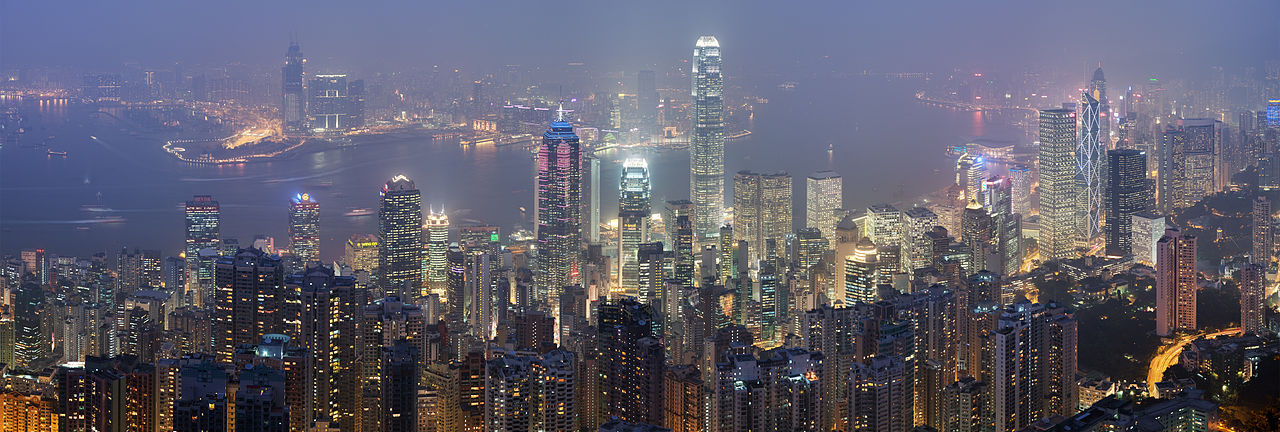
\includegraphics[width=\paperwidth]{hong_kong}};
\tikz[overlay,remember picture]\node[anchor=south east, fill=white,
inner sep=.3mm] at (current page.south east) {%
\tiny David Iliff, CC-BY-SA};
\end{frame}

\begin{frame}
  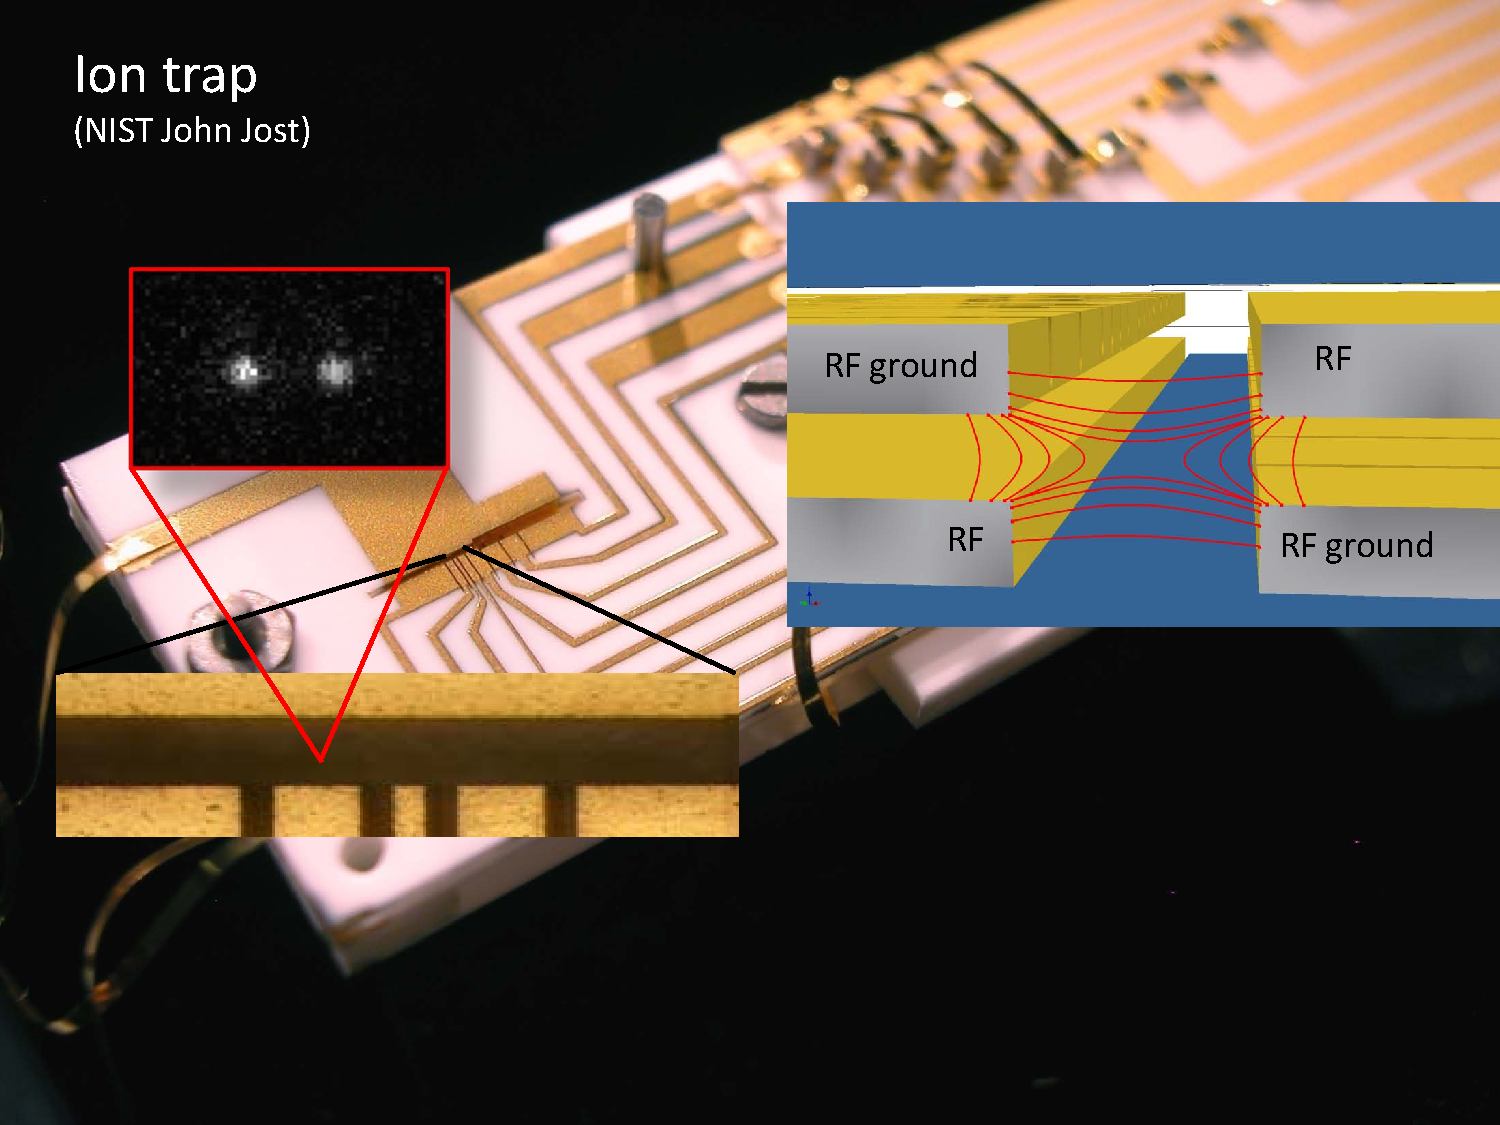
\includegraphics[width=\columnwidth]{jost_trap-3}
\end{frame}

\begin{frame}
  \frametitle{Quantum gate sequences (NIST)}
  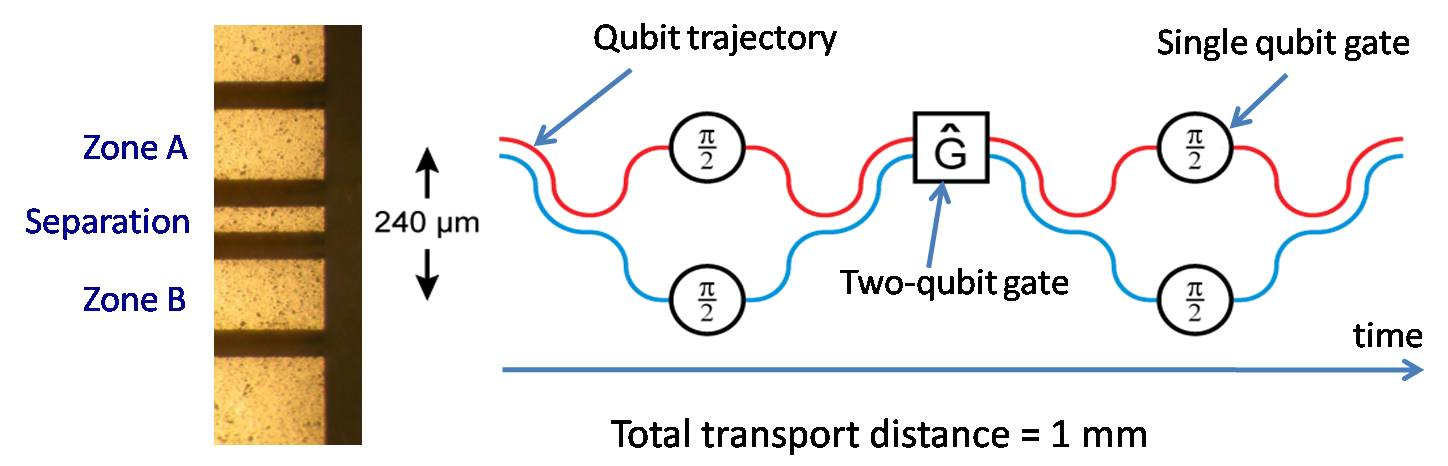
\includegraphics[width=\columnwidth]{gate_sequence}
\end{frame}

\begin{frame}
  \begin{tikzpicture}[box/.style={rectangle,fill=white}]
    \node[inner sep=0] {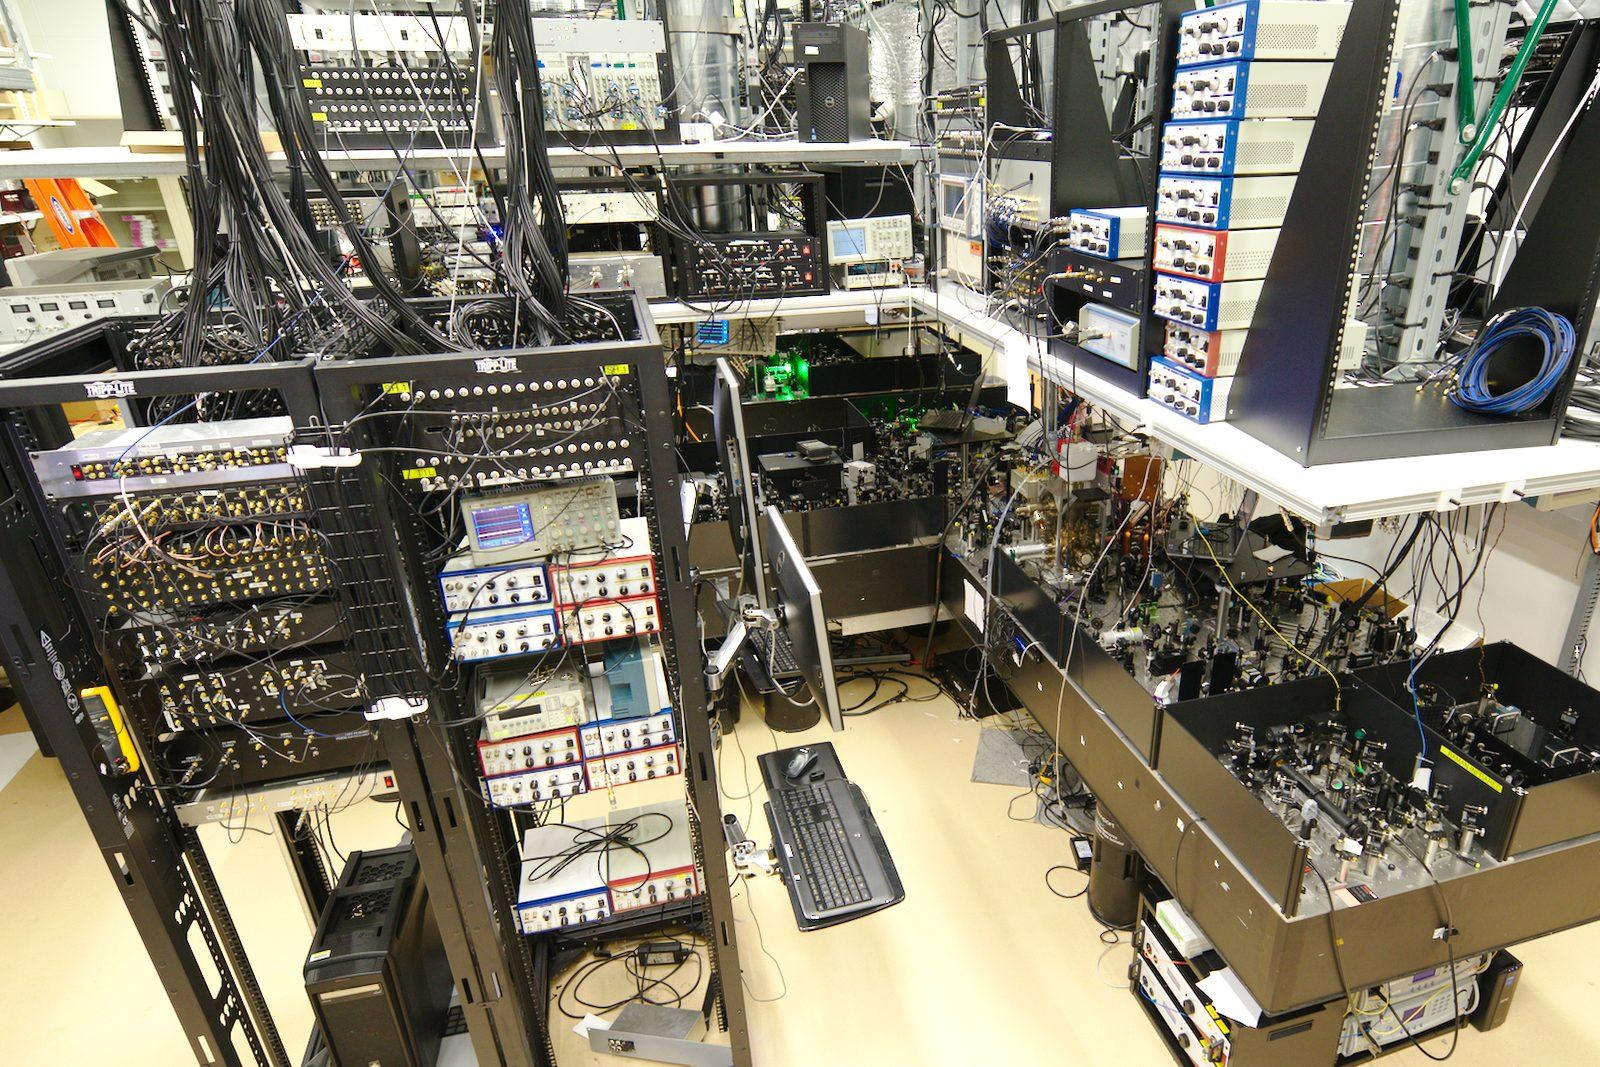
\includegraphics[width=\columnwidth]{lab}};\pause
    %\draw[help lines,white] (-4, -3) grid (4, 3);
    \node[box] at (-4, -2) {FPGA};
    \node[box] at (3.5, 0) {ion trap};
    \node[box] at (-3, 3) {$\sim$10 attenuators};
    \node[box] at (2, 2) {$\sim$50 DAC};
    \node[box] at (-4, 0) {$\sim$20 DDS};
    \node[box] at (-2, 1) {$\sim$50 GPIO};
    \node[box] at (.5, 0) {$\sim$10 motors};
    \node[box] at (2, -2) {$\sim$10 power supplies};
    \node[box] at (4, -3) {$\sim$10 lasers};
  \end{tikzpicture}
\end{frame}

\begin{frame}
  \frametitle{Enter ARTIQ}
  \alert{A}dvanced \alert{R}eal-\alert{T}ime \alert{I}nfrastructure for \alert{Q}uantum physics

  \footnotesize
  \begin{itemize}
    \item High performance --- nanosecond resolution, hundreds of ns latency
    \item Expressive --- describe algorithms with few lines of code
    \item Portable --- treat hardware, especially FPGA boards, as commodity
    \item Modular --- separate components as much as possible
    \item Flexible --- hard-code as little as possible
  \end{itemize}
\end{frame}

\begin{frame}[fragile]
  \frametitle{Define a simple timing language}
  \footnotesize

  \begin{minted}[frame=leftline]{python}
trigger.sync()                # wait for trigger input
start = now()                 # capture trigger time
for i in range(3):
    delay(5*us)
    dds.pulse(900*MHz, 7*us)  # first pulse 5 µs after trigger
at(start + 1*ms)              # re-reference time-line
dds.pulse(200*MHz, 11*us)     # exactly 1 ms after trigger
  \end{minted}

  \begin{itemize}
    \item Written in a subset of Python
    \item Executed on a CPU embedded on a FPGA (the \emph{core device})
    \item \verb!now(), at(), delay()! describe time-line of an experiment
    \item Exact time is kept in an internal variable
    \item That variable only loosely tracks the execution time of CPU instructions
    \item The value of that variable is exchanged with the RTIO fabric that
      does precise timing
  \end{itemize}
\end{frame}


\begin{frame}[fragile]
  \frametitle{Convenient syntax additions}
  \footnotesize
  \begin{minted}[frame=leftline]{python}
with sequential:
    with parallel:
        a.pulse(100*MHz, 10*us)
        b.pulse(200*MHz, 20*us)
    with parallel:
        c.pulse(300*MHz, 30*us)
        d.pulse(400*MHz, 20*us)
  \end{minted}

  \begin{itemize}
    \item Experiments are inherently parallel:
        simultaneous laser pulses, parallel cooling of ions in different trap zones
    \item \verb!parallel! and \verb!sequential! contexts with arbitrary nesting
    \item \verb!a! and \verb!b! pulses both start at the same time
    \item \verb!c! and \verb!d! pulses both start when \verb!a! and \verb!b! are both done
      (after 20\,µs)
    \item Implemented by inlining, loop-unrolling, and interleaving
  \end{itemize}
\end{frame}


\begin{frame}[fragile]
  \frametitle{Physical quantities, hardware granularity}
  \footnotesize
  \begin{minted}[frame=leftline]{python}
n = 1000
dt = 1.2345*ns
f = 345*MHz

dds.on(f, phase=0)              # must round to integer tuning word
for i in range(n):
    delay(dt)                   # must round to native cycles

dt_raw = time_to_cycles(dt)     # integer number of cycles
f_raw = dds.frequency_to_ftw(f) # integer frequency tuning word

# determine correct phase despite accumulation of rounding errors
phi = n*cycles_to_time(dt_raw)*dds.ftw_to_frequency(f_raw)
  \end{minted}

  \begin{itemize}
    \item Need well defined conversion and rounding of physical quantities
      (time, frequency, phase, etc.) to hardware granularity and back
    \item Complicated because of calibration, offsets, cable delays,
      non-linearities
    \item No generic way to do it automatically and correctly
    \item $\rightarrow$ need to do it explicitly where it matters
  \end{itemize}
\end{frame}


\begin{frame}[fragile]
  \frametitle{Invite organizing experiment components and code reuse}
  \footnotesize

  \begin{minted}[frame=leftline]{python}
class Experiment:
    def build(self):
        self.ion1 = Ion(...)
        self.ion2 = Ion(...)
        self.transporter = Transporter(...)

    @kernel
    def run(self):
        with parallel:
          self.ion1.cool(duration=10*us)
          self.ion2.cool(frequency=...)
        self.transporter.move(speed=...)
        delay(100*ms)
        self.ion1.detect(duration=...)
  \end{minted}
\end{frame}


\begin{frame}[fragile]
  \frametitle{RPC to handle distributed non-RT hardware}
  \footnotesize

  \begin{minted}[frame=leftline]{python}
class Experiment:
    def prepare(self):              # runs on the host
        self.motor.move_to(20*mm)   # slow RS232 motor controller

    @kernel
    def run(self):                  # runs on the RT core device
        self.prepare()              # converted into an RPC
  \end{minted}

  \begin{itemize}
    \item When a kernel function calls a non-kernel function, it generates a RPC
    \item The callee is executed on the host
    \item Mechanism to report results and control slow devices
    \item The kernel must have a loose real-time constraint (a long \verb!delay!)
        or means of re-synchronization to cover communication, host, and device delays
  \end{itemize}
\end{frame}


\begin{frame}
  \frametitle{Kernel deployment to the core device}
  \footnotesize
  \begin{itemize}
    \item RPC and exception mappings are generated
    \item Constants and small kernels are inlined
    \item Small loops are unrolled
    \item Statements in parallel blocks are interleaved
    \item Time is converted to RTIO clock cycles
    \item The Python AST is converted to LLVM IR
    \item The LLVM IR is compiled to OpenRISC machine code
    \item The OpenRISC binary is sent to the core device
    \item The runtime in the core device links and runs the kernel
    \item The kernel calls the runtime for communication (RPC) and interfacing
      with core device peripherals (RTIO, DDS)
  \end{itemize}
\end{frame}


\begin{frame}
  \frametitle{Higher level features}
  \footnotesize
  \begin{itemize}
  \item Device management: drivers, remote devices, device database
  \item Parameter database \\
       e.g.\ ion properties such as qubit flopping frequency
  \item Scheduling of experiments \\
      e.g.\ calibrations, queue
  \item Archival of results (HDF5 format)
  \item Graphical user interface \\ 
  	run with arguments, schedule, real-time plotting
  \end{itemize}
\end{frame}


\begin{frame}
  \frametitle{Short-term hardware support}
  \footnotesize
  \begin{itemize}
  \item Core device: Papilio Pro, Pipistrello, KC705
  \item High speed DDS with AD9858 and AD9914 \\
  	(direct core device, $ < 25$ channels)
  \item Waveform generation: PDQ (NIST), PXI6733
  \item Lab Brick Digital Attenuators
  \item Novatech 409B DDS
  \item Thorlabs motor controllers
  \end{itemize}
\end{frame}  

\begin{frame}
  \begin{center}
  
\includegraphics[width=3cm]{../../logo/artiq.pdf} \\
  \url{http://m-labs.hk/artiq}
  \end{center}

  \footnotesize
  \begin{itemize}
    \item Public mailing list (with archives)
    \item Full source code, BSD licensed
    \item Design applicable beyond ion trapping (superconducting qubits,
      neutral atoms...)
  \end{itemize}
  \textit{Thanks to Robert J\"ordens, Joe Britton, Daniel Slichter and other members of the NIST Ion Storage Group for their support in developing ARTIQ.}

\end{frame}

\end{document}
